% Лабораторная работа 3, часть 2 — постер (tikzposter)
% Компилировать LuaLaTeX.
\documentclass[25pt, a0paper, portrait, margin=0mm, innermargin=15mm,
               blockverticalspace=25mm, colspace=15mm, subcolspace=8mm]{tikzposter}

% --- шрифты и язык ---
\usepackage{fontspec}
\defaultfontfeatures{Renderer=Basic, Ligatures=TeX}
\newfontfamily\cyrillicfonttt{CMU Typewriter Text}
\newfontfamily\cyrillicfont{CMU Sans Serif}
\newfontfamily\cyrillicfontsf{CMU Sans Serif}
\setmainfont{CMU Sans Serif}
\setsansfont{CMU Sans Serif}
\setmonofont{CMU Typewriter Text}

\usepackage{polyglossia}
\setdefaultlanguage{russian}
\setotherlanguages{english}

% --- пакеты ---
\usepackage{graphicx}
\usepackage{booktabs}
\usepackage{array}
\usepackage{url}
\newcommand{\q}{\symbol{34}}
\usetikzlibrary{positioning, arrows.meta, shapes.multipart}

% --- тема и цвета ---
\usetheme{Simple}
\usecolorstyle[colorPalette=BlueGrayOrange]{Default}
\useblockstyle{Default}
% свои цвета поверх палитры
\colorlet{backgroundcolor}{colorTwo!10}
\colorlet{titlebgcolor}{colorOne}
\colorlet{titlefgcolor}{white}
\colorlet{blocktitlebgcolor}{colorOne}
\colorlet{blocktitlefgcolor}{white}
\colorlet{blockbodybgcolor}{white}
\colorlet{blockbodyfgcolor}{black}

% --- титульные данные ---
\title{Асинхронный REST API курсов валют ЦБ РФ}
\author{Фролов А.\,А., группа ИВТ-2.3}
\institute{РГПУ им.~А.\,И.~Герцена, Институт информационных технологий и технологического образования}

\begin{document}
\maketitle

\begin{columns}

% ================= Левая колонка =================
\column{0.5}

\block{Аннотация}{
  Разработан веб-сервис для получения и хранения курсов валют Центрального
  банка Российской Федерации. Сервис построен на асинхронном фреймворке
  FastAPI, хранит данные в SQLite через асинхронный SQLAlchemy и позволяет
  пользователям подписываться на интересующие валюты. В работе описаны
  архитектура приложения, структура базы данных и набор эндпоинтов API.
}

\block{Введение}{
  Курсы валют нужны во многих приложениях: от интернет-магазинов до
  финансовых сервисов. Банк России публикует официальные курсы в открытом
  доступе, но удобнее работать с ними через собственный API, который
  хранит данные и знает о пользователях.

  \vspace{0.5em}
  \textbf{Цель:} разработать REST API для работы с курсами валют ЦБ РФ.

  \vspace{0.5em}
  \textbf{Задачи:}
  \begin{itemize}
    \item спроектировать базу данных;
    \item реализовать CRUD-операции для пользователей;
    \item загружать курсы валют из API Банка России;
    \item реализовать подписки пользователей на валюты.
  \end{itemize}
}

\block{Методы}{
  \textbf{Стек:} Python, FastAPI, SQLAlchemy (async), Pydantic, SQLite.

  \vspace{0.5em}
  Код разделён на слои: \texttt{routers} принимают запросы,
  \texttt{services} содержат бизнес-логику, \texttt{models} описывают
  таблицы, \texttt{schemas} проверяют входные и выходные данные.

  \vspace{1em}
  \begin{center}
  \begin{tikzpicture}[scale=1.3, transform shape,
      box/.style={draw=blocktitlebgcolor, very thick, rounded corners=8pt,
                  fill=white, minimum width=12cm, minimum height=2.4cm,
                  font=\Large, align=center},
      ext/.style={box, draw=orange!80!black, fill=orange!10, minimum width=9cm},
      >={Stealth[length=6mm]}, node distance=1.4cm]
    \node[box] (client)   {Клиент\\ \normalsize HTTP-запрос};
    \node[box, below=of client]   (routers)  {routers\\ \normalsize эндпоинты FastAPI};
    \node[box, below=of routers]  (services) {services\\ \normalsize бизнес-логика};
    \node[box, below=of services] (db)       {SQLite\\ \normalsize через SQLAlchemy};
    \node[ext, right=2.5cm of services] (cbr) {API Банка России\\ \normalsize курсы валют};
    \draw[->, ultra thick] (client) -- (routers);
    \draw[->, ultra thick] (routers) -- node[right, font=\normalsize] {Pydantic} (services);
    \draw[->, ultra thick] (services) -- node[right, font=\normalsize] {async} (db);
    \draw[->, ultra thick] (services) -- node[above, font=\normalsize] {HTTP} (cbr);
  \end{tikzpicture}

  \vspace{0.5em}
  \normalsize Рис.~1. Архитектура приложения
  \end{center}
}

\block{Интерфейс API}{
  FastAPI сам строит документацию по коду. По адресу \texttt{/docs}
  открывается Swagger UI, где каждый эндпоинт можно вызвать из браузера.

  \vspace{0.5em}
  \begin{center}
  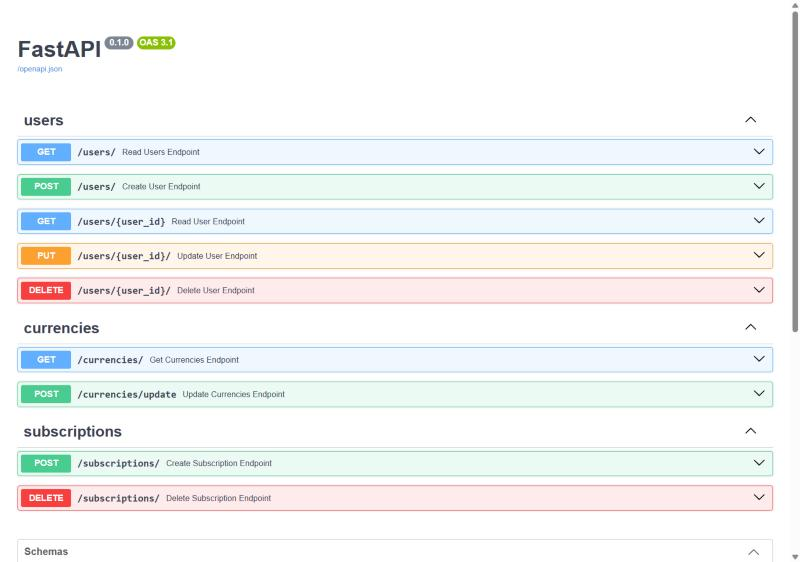
\includegraphics[width=0.6\linewidth]{swagger}

  \vspace{0.5em}
  \normalsize Рис.~2. Swagger UI сервиса
  \end{center}
}

% ================= Правая колонка =================
\column{0.5}

\block{Результаты}{
  \textbf{Структура базы данных.} Три таблицы; подписка связывает
  пользователя и валюту (связи «один ко многим»).

  \vspace{1em}
  \begin{center}
  \begin{tikzpicture}[scale=1.45, transform shape,
      table/.style={rectangle split, rectangle split parts=2, draw=blocktitlebgcolor,
                    very thick, rounded corners=6pt, font=\large, align=left,
                    rectangle split part fill={blocktitlebgcolor!25, white},
                    minimum width=8cm, inner sep=10pt},
      >={Stealth[length=6mm]}]
    \node[table] (user) {\textbf{User}
      \nodepart{second} id\\ username\\ email\\ created\_at};
    \node[table, right=5cm of user] (sub) {\textbf{Subscription}
      \nodepart{second} id\\ user\_id\\ currency\_id};
    \node[table, below=2.5cm of sub] (cur) {\textbf{Currency}
      \nodepart{second} id\\ code\\ name\\ value};
    \draw[->, ultra thick] (user) -- node[above, font=\large] {1 : N} (sub);
    \draw[->, ultra thick] (cur) -- node[right, font=\large] {1 : N} (sub);
  \end{tikzpicture}

  \vspace{0.5em}
  \normalsize Рис.~3. Схема базы данных
  \end{center}

  \vspace{1em}
  \textbf{Эндпоинты API.}

  \vspace{0.5em}
  \begin{center}
  \begin{tabular}{l>{\raggedright\arraybackslash}p{0.62\linewidth}}
    \toprule
    \textbf{Ресурс} & \textbf{Операции} \\
    \midrule
    \texttt{/users/}        & создание, список, просмотр, изменение, удаление \\
    \texttt{/currencies/}   & получение курсов, синхронизация с ЦБ РФ \\
    \texttt{/subscriptions/} & оформление и отмена подписки \\
    \bottomrule
  \end{tabular}
  \end{center}

  \vspace{0.5em}
  Все операции с базой данных выполняются асинхронно, входные данные
  проверяются схемами Pydantic.
}

\block{Пример ответа}{
  Запрос \texttt{GET /currencies/} после синхронизации с ЦБ РФ возвращает
  список валют с курсом в рублях:

  \vspace{0.5em}
  {\ttfamily\addfontfeatures{Ligatures=TeXOff}\normalsize
  [\\
  \hspace*{1.5em}\{\q id\q: 1, \q code\q: \q AUD\q, \q name\q: \q Австралийский доллар\q, \q value\q: 57.1567\},\\
  \hspace*{1.5em}\{\q id\q: 4, \q code\q: \q GBP\q, \q name\q: \q Фунт стерлингов\q, \q value\q: 110.6399\},\\
  \hspace*{1.5em}...\\
  ]\par}
}

\block{Выводы}{
  \begin{itemize}
    \item Реализован асинхронный REST API на FastAPI и SQLAlchemy.
    \item Настроена загрузка официальных курсов из API Банка России.
    \item Спроектирована база данных из трёх связанных таблиц.
    \item Разделение кода на слои упрощает поддержку и расширение.
    \item Дальнейшее развитие: тесты, аутентификация, развёртывание в Docker.
  \end{itemize}
}

\block{Список литературы}{
  \raggedright
  \begin{enumerate}
    \item FastAPI Documentation. \url{https://fastapi.tiangolo.com/}
    \item SQLAlchemy 2.0 Documentation: Asynchronous I/O.
          \url{https://docs.sqlalchemy.org/en/20/orm/extensions/asyncio.html}
    \item Pydantic Documentation. \url{https://docs.pydantic.dev/}
    \item Банк России. Получение данных с использованием XML.
          \url{https://www.cbr.ru/development/SXML/}
    \item Исходный код проекта. \url{https://github.com/bluv4nul/cbrrf-rest-api}
  \end{enumerate}
}

\end{columns}

\end{document}
